% !TEX program = lualatex
\documentclass[11pt,twoside]{article}
\usepackage{apuntes-oscuro}

\asignatura{Ecuaciones Diferenciales}
\cabecera{Tema 4\ \ ·\ \ EDO lineales de orden superior}
\hypersetup{pdftitle={Tema 4. Parte II. Coeficientes indeterminados, Cauchy-Euler y oscilador forzado},
  pdfauthor={Daniel Martín Guerrero}}

% ---------- notación propia (coherente con la parte I) ----------
\newcommand\Lop{\mathcal L}
\newcommand\yh{\hat y}
\newcommand\vyh{\hat{\bm y}}
\newcommand\vk{\bm k}
\newcommand\D{D}
\newcommand\abs[1]{\lvert#1\rvert}
\newcommand\mat[1]{\begin{pmatrix}#1\end{pmatrix}}
\newcommand\smat[1]{\left(\begin{smallmatrix}#1\end{smallmatrix}\right)}
\providecommand\senh{\operatorname{senh}}
% referencia a la parte I: \pI{4.9} -> (P1, 4.9)
\newcommand\pI[1]{(P1,~#1)}
\renewcommand\thesection{\arabic{section}}

\begin{document}

% =====================================================================
%  PORTADA
% =====================================================================
\setcounter{page}{31}
\begin{titlepage}
\setcounter{page}{31}
\thispagestyle{empty}
\centering
\vspace*{-0.6cm}

\includegraphics[width=4.6cm]{figuras/usal.png}\par
\vspace{0.75cm}
{\color{sky}\rule{\textwidth}{0.5pt}}\par
\vspace{0.55cm}
{\color{muted}\small\textls[220]{\textsc{Facultad de Ciencias}}\quad·\quad\textls[220]{\textsc{Grado en Física}}}\par
\vspace{1.25cm}
{\color{acc}\textls[260]{\textsc{Ecuaciones Diferenciales}}}\par
\vspace{0.2cm}
{\color{muted}\small\textls[260]{\textsc{Tema 4\ \ ·\ \ Parte II}}}\par
\vspace{1.25cm}
{\fontsize{27}{33}\selectfont\bfseries EDO lineales de orden superior\par}
\vspace{0.12cm}
{\fontsize{19}{24}\selectfont\bfseries fuentes, coeficientes variables y resonancia\par}
\vspace{0.55cm}
{\color{acc}\rule{2.4cm}{0.8pt}}\par
\vspace{0.45cm}
{\color{muted}\small\itshape Variación de las constantes en orden tres\quad·\quad Coeficientes indeterminados\quad·\quad Anuladores\par
Ecuación de Cauchy--Euler\quad·\quad Reducción de orden\quad·\quad Oscilador forzado y resonancia\par}
\vspace{0.45cm}
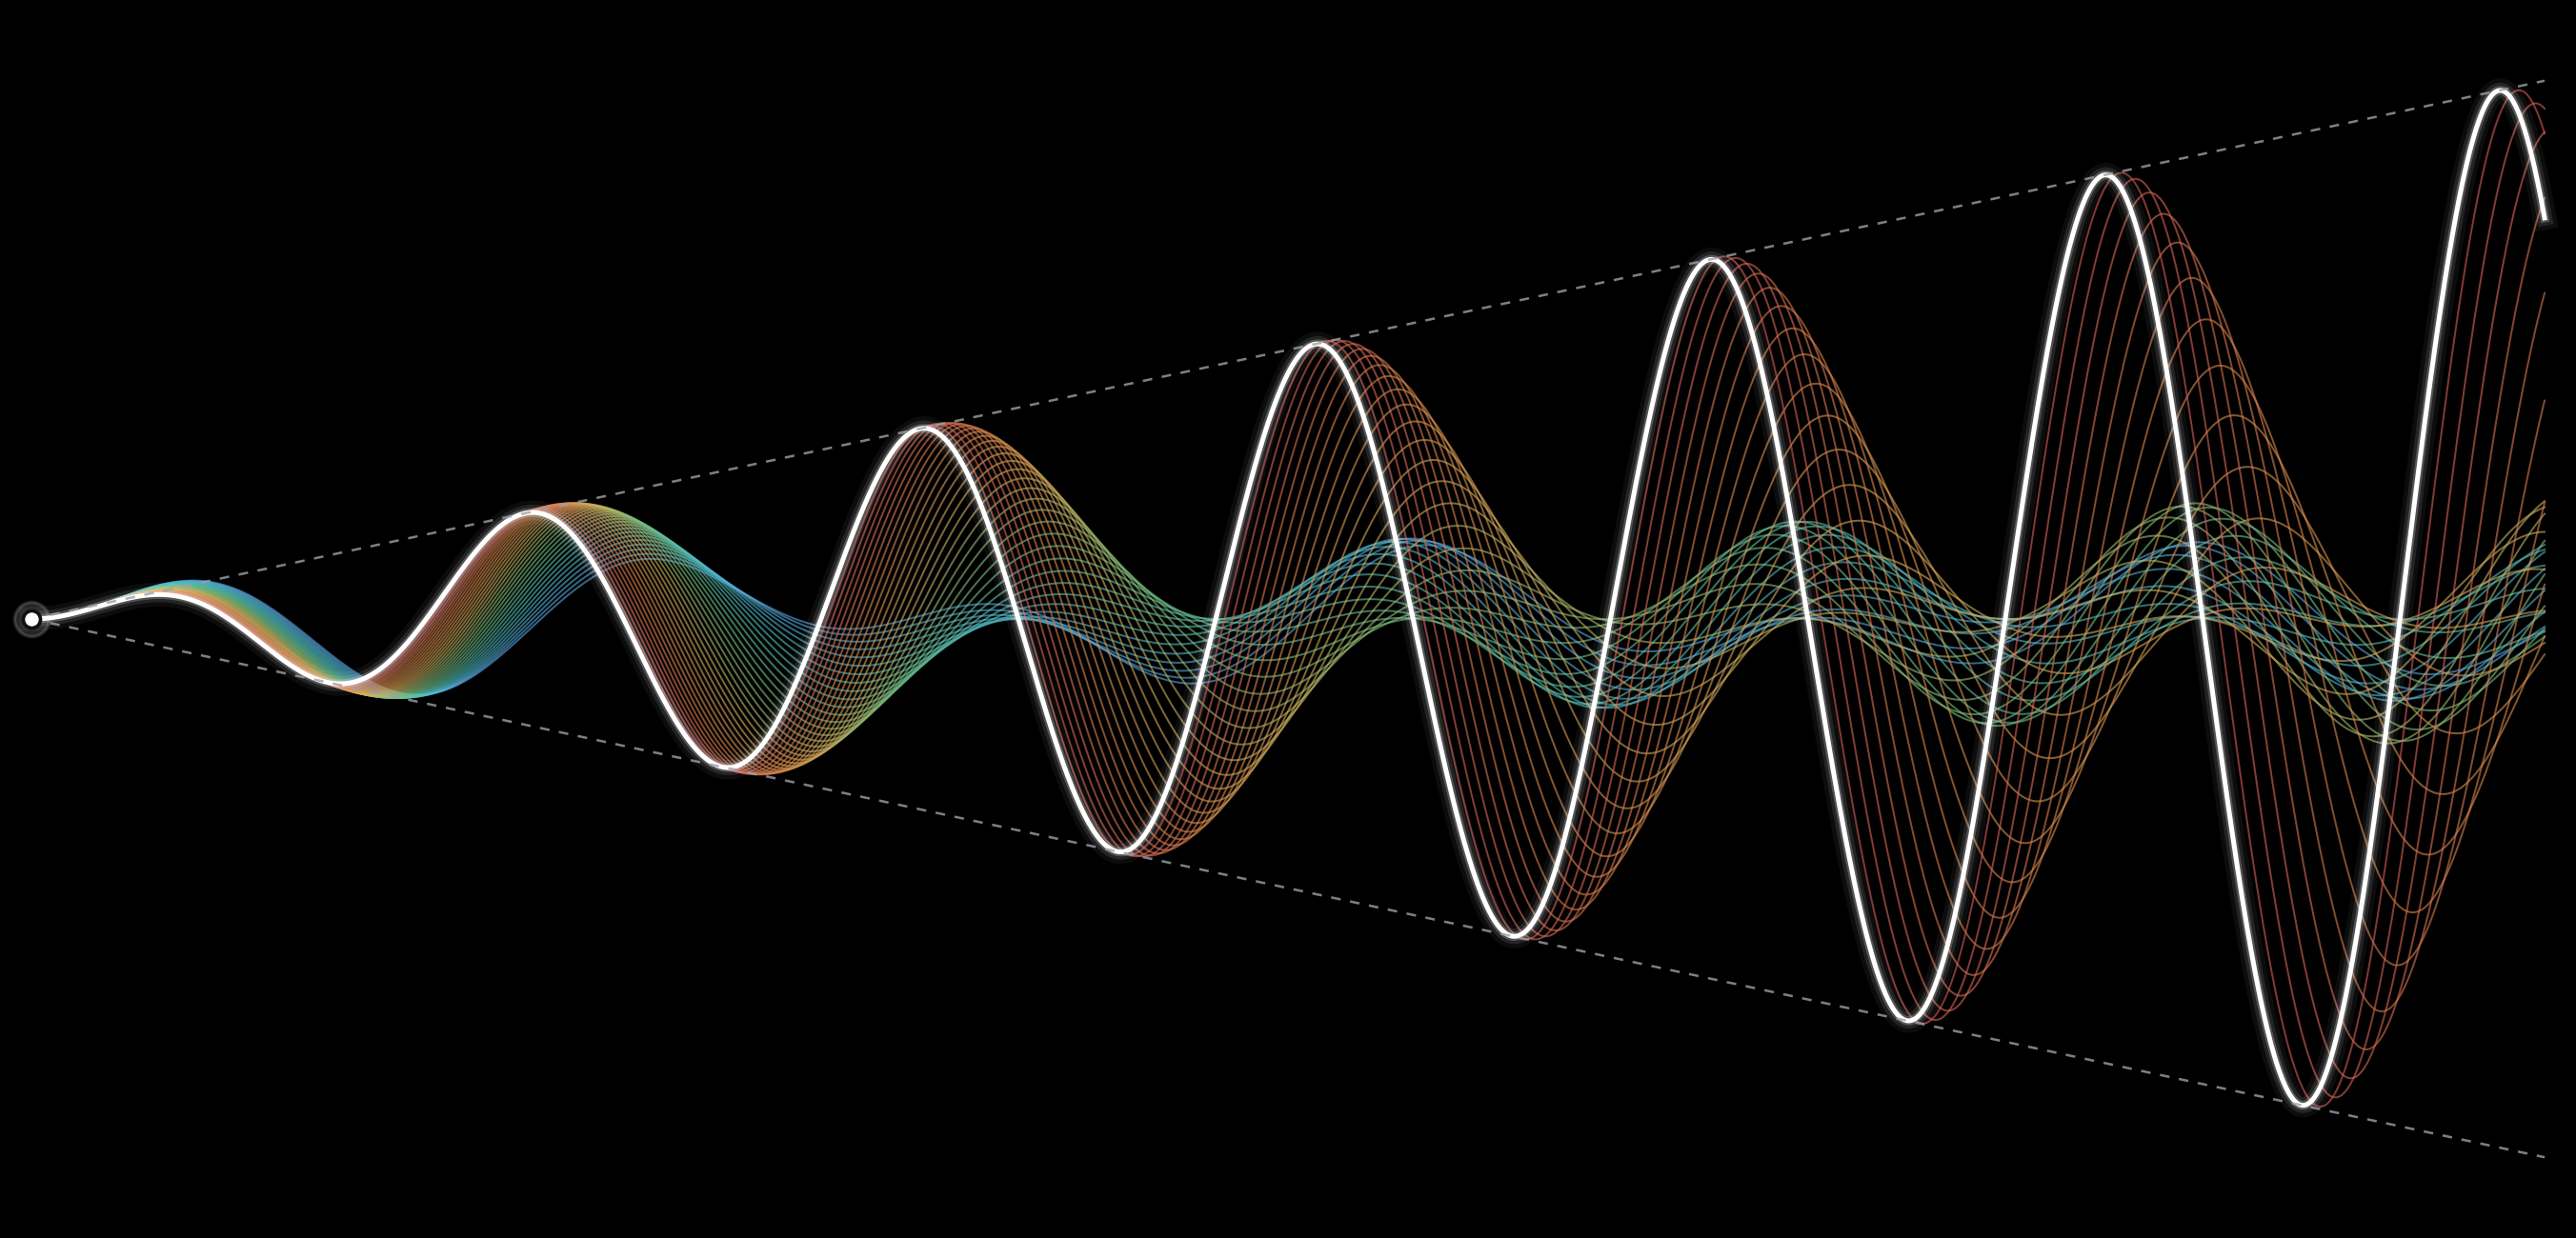
\includegraphics[width=0.86\textwidth]{figuras/portada_t4.png}\par
\vspace{0.35cm}
{\small$\displaystyle x''+\omega^2x=\frac{F_0}{m}\cos\Omega t\quad\xrightarrow{\ \Omega\to\omega\ }\quad
x_p(t)=\frac{F_0}{2m\omega}\,t\,\sen\omega t$\par}
\vfill
{\color{sky}\rule{\textwidth}{0.5pt}}\par
\vspace{0.3cm}
\begin{minipage}[t]{0.32\textwidth}\raggedright
{\color{acc}\footnotesize\textls[200]{\textsc{Autor}}}\par\vspace{2pt}
{\small Daniel Martín Guerrero}
\end{minipage}\hfill
\begin{minipage}[t]{0.32\textwidth}\centering
{\color{acc}\footnotesize\textls[200]{\textsc{Profesorado}}}\par\vspace{2pt}
{\small Pilar García Estévez\\ José Beltrán Jiménez\\ María Pérez Garrote}
\end{minipage}\hfill
\begin{minipage}[t]{0.32\textwidth}\raggedleft
{\color{acc}\footnotesize\textls[200]{\textsc{Apuntes formalizados}}}\par\vspace{2pt}
{\small Salamanca, curso 2026/2027}\\[1pt]
{\footnotesize\color{muted}Teoría y seminario de problemas}
\end{minipage}
\end{titlepage}

% =====================================================================
%  ÍNDICE
% =====================================================================
\setcounter{page}{32}
{\hypersetup{linkcolor=fg}\tableofcontents}
\clearpage

% =====================================================================
\section{De la parte I a la parte II}\label{sec:intro}
% =====================================================================

\begin{motivacion}{Plan de la parte II}
La parte I construyó la base de $\ker\Lop$ con coeficientes constantes y dio dos fórmulas generales para la
particular: variación de las constantes \pI{4.9} y la función de Green \pI{5.7}. Aquí las hacemos operativas.
Empezamos con un ejemplo de orden tres por variación de las constantes (sección~\ref{sec:orden3}); después
vemos el atajo de los \emph{coeficientes indeterminados}, justificado con anuladores (sección~\ref{sec:coefind}); la
ecuación de \emph{Cauchy--Euler}, que se reduce a coeficientes constantes con $x=\e^t$ (sección~\ref{sec:euler}); la
\emph{reducción de orden} (sección~\ref{sec:reduccion}), y el \emph{oscilador forzado} con su resonancia
(sección~\ref{sec:oscilador}). Cerramos con el puente al tema~6 y el seminario.
\end{motivacion}

\begin{observacion}[notación]
Seguimos la de la parte I: $\Lop=\sum_ja_j(x)\,\D^j$ con $\D=\dd/\dd x$, $\{\yh_1,\dots,\yh_n\}$ sistema fundamental,
$W$ matriz wronskiana, $w=\det W$, $\bm e_n=(0,\dots,0,1)\T$ y $\Theta$ la función escalón. Los resultados de la
parte I se citan como \pI{4.9}, \pI{teorema~3.5}, etc.
\end{observacion}

Recordamos las dos herramientas que más usaremos.
\begin{itemize}
\item \emph{Conjugación por la exponencial} \pI{lema~3.1}: para todo polinomio $p$,
\begin{equation}\label{eq:conj}
p(\D)\big[\e^{\lambda x}g(x)\big]=\e^{\lambda x}\,p(\D+\lambda)\,g(x),\qquad\text{en particular}\quad
(\D-\lambda)^m\big[\e^{\lambda x}g\big]=\e^{\lambda x}g^{(m)} .
\end{equation}
\item \emph{Variación de las constantes} \pI{4.9}: $y_p(x)=\vyh\T(x)\int_{x_0}^{x}W^{-1}(s)\,\bm e_n\,\dfrac{b(s)}{a_n(s)}\,\dd s$; para
$n=2$,
\begin{equation}\label{eq:vc2}
y_p(x)=\int_{x_0}^{x}\frac{\yh_1(s)\,\yh_2(x)-\yh_1(x)\,\yh_2(s)}{w(s)}\,\frac{b(s)}{a_2(s)}\,\dd s .
\end{equation}
\end{itemize}

% =====================================================================
\section{Variación de las constantes en orden tres}\label{sec:orden3}
% =====================================================================

\begin{ejemplo}[$4y'''+4y'=\tan x$, $\ \abs x<\pi/2$]\label{ej:tan}
\begin{pasos}
\item \emph{Homogénea.} $p(\lambda)=4\lambda^3+4\lambda=4\lambda(\lambda^2+1)\Rightarrow\lambda=0,\pm\iu$, y
$y_h=c_1+c_2\sen x+c_3\cos x$.
\item \emph{Wronskiano} de $\vyh=(1,\sen x,\cos x)\T$:
\begin{equation*}
W=\mat{1&\sen x&\cos x\\0&\cos x&-\sen x\\0&-\sen x&-\cos x},\qquad
W^{-1}=\mat{1&0&1\\0&\cos x&-\sen x\\0&-\sen x&-\cos x}.
\end{equation*}
con $w=\det W=-\cos^2x-\sen^2x=-1$. (Curiosamente, $W^{-1}$ coincide con $W$ salvo en la primera fila: compruébese $WW^{-1}=\Id$.)
\item \emph{Sistema para $\vk\,'$.} Sólo hace falta la última columna de $W^{-1}$, y $b/a_3=\tfrac14\tan x$:
\begin{equation*}
\vk\,'=W^{-1}\bm e_3\,\frac{\tan x}{4}=\frac{\tan x}{4}\mat{1\\-\sen x\\-\cos x}
\quad\Longrightarrow\quad
\begin{cases}k_1'=\dfrac{\tan x}{4},\\[4pt] k_2'=-\dfrac{\sen^2x}{4\cos x},\\[4pt] k_3'=-\dfrac{\sen x}{4}.\end{cases}
\end{equation*}
\item \emph{Integrales.} Con $\int\tan x\,\dd x=-\ln\cos x$ y $\dfrac{\sen^2x}{\cos x}=\dfrac1{\cos x}-\cos x$,
$\ \int\dfrac{\dd x}{\cos x}=\ln(\sec x+\tan x)$:
\begin{equation*}
k_1=-\tfrac14\ln\cos x,\qquad k_2=-\tfrac14\big[\ln(\sec x+\tan x)-\sen x\big],\qquad k_3=\tfrac14\cos x .
\end{equation*}
\item \emph{Particular.} $y_p=k_1\cdot1+k_2\sen x+k_3\cos x
=-\tfrac14\ln\cos x-\tfrac14\sen x\ln(\sec x+\tan x)+\tfrac14\big(\sen^2x+\cos^2x\big)$. La constante $\tfrac14$ es homogénea:
\begin{equation}\label{eq:tan}
\res{y=c_1+c_2\sen x+c_3\cos x-\frac14\Big[\ln\cos x+\sen x\,\ln\frac{1+\sen x}{\cos x}\Big]}
\end{equation}
\end{pasos}
\end{ejemplo}

\begin{observacion}[errata del manuscrito]
En los apuntes de clase el resultado aparece como $-\frac14\ln\frac{1+\sen x}{\cos x}+\frac{\sen x}4+\frac{\cos x}4-\frac14\ln\cos x$:
falta multiplicar cada $k_i$ por su $\yh_i$. Al hacerlo, el logaritmo lleva el factor $\sen x$ y los términos
$\frac{\sen x}4,\frac{\cos x}4$ se convierten en $\frac{\sen^2x+\cos^2x}{4}=\frac14$. Sustituyendo la versión del
manuscrito en la ecuación sobra $-2/[(1+\sen x)\cos x]$; \eqref{eq:tan} la cumple exactamente.
\end{observacion}

\begin{consejo}{Atajo con la función de Green}
Con coeficientes constantes, $G(x,s)$ es la solución homogénea con datos $(0,\dots,0,1/a_n)$ en $s$ \pI{5.7}. Para
$\D^3+\D$ basta mirar la base: $g(x)=1-\cos(x-s)$ cumple $g(s)=0$, $g'(s)=\sen0=0$, $g''(s)=\cos0=1$. Luego
$y_p=\frac14\int_0^x\big[1-\cos(x-s)\big]\tan s\,\dd s$, sin invertir $W$ (problema~\ref{prob:5}).
\end{consejo}

% =====================================================================
\section{Método de los coeficientes indeterminados}\label{sec:coefind}
% =====================================================================

La variación de las constantes vale siempre, pero obliga a integrar. Si $\Lop$ tiene coeficientes constantes y la
fuente es de un tipo concreto, podemos adivinar la forma de $y_p$ y sólo hay que resolver un sistema lineal.

\subsection{Fuentes admisibles y ansatz}

\begin{definicion}[Fuente cuasipolinómica]\label{def:fuente}
Una fuente es \emph{admisible} si
\begin{equation}\label{eq:fuente}
b(x)=\e^{\alpha x}\big[P(x)\cos\beta x+Q(x)\sen\beta x\big],\qquad \alpha,\beta\in\R,\quad \deg P=r,\ \deg Q=s .
\end{equation}
Incluye polinomios ($\alpha=\beta=0$), exponenciales ($\beta=0$, $P$ constante) y senos y cosenos ($\alpha=0$).
Llamamos $\mu\defeq\alpha+\iu\beta$ al \emph{exponente} de la fuente y $m\defeq\max(r,s)$.
\end{definicion}

\begin{teorema}[Ansatz de coeficientes indeterminados]\label{teo:ansatz}
Sea $\Lop=p(\D)$ con coeficientes constantes y $b$ como en \eqref{eq:fuente}. Sea $h\ge0$ la multiplicidad de $\mu$
como raíz de $p$ ($h=0$ si no lo es). Entonces existe una solución particular de la forma
\begin{equation}\label{eq:ansatz}
\res{y_p(x)=x^{h}\,\e^{\alpha x}\big[\hat P(x)\cos\beta x+\hat Q(x)\sen\beta x\big],\qquad \deg\hat P,\ \deg\hat Q\le m}
\end{equation}
cuyos $2(m+1)$ coeficientes (o $m+1$ si $\beta=0$) se obtienen sustituyendo e igualando.
\end{teorema}

El factor $x^h$ es la \emph{resonancia}: si la fuente «se parece» a una solución homogénea, el ansatz sin $x^h$
cae en $\ker\Lop$ y no puede producir $b$.

\subsection{Justificación: el método del anulador}

\begin{definicion}[Anulador]
Un polinomio $M(\D)$ \emph{anula} $b$ si $M(\D)\,b=0$. Por \pI{proposición~3.3} y \pI{proposición~2.8},
\begin{equation}\label{eq:anulador}
M(\D)=\begin{cases}(\D-\alpha)^{m+1}, & \beta=0,\\[2pt] \big[(\D-\alpha)^2+\beta^2\big]^{m+1}=\big[(\D-\mu)(\D-\mu^*)\big]^{m+1}, & \beta\neq0,\end{cases}
\end{equation}
anula \eqref{eq:fuente}, porque $\ker(\D-\mu)^{m+1}=\spn\{x^k\e^{\mu x}\}_{k\le m}$.
\end{definicion}

\begin{demostracion}[del teorema~\ref{teo:ansatz}]
\begin{pasos}
\item \emph{Aplicamos el anulador.} Si $p(\D)y_p=b$, entonces $M(\D)\,p(\D)\,y_p=M(\D)\,b=0$: $y_p$ resuelve una ecuación
\emph{homogénea} de coeficientes constantes, de polinomio $M\,p$.
\item \emph{Multiplicidades.} En $M\,p$, la raíz $\mu$ tiene multiplicidad $h+m+1$. Por \pI{teorema~3.5}, $y_p$ es
combinación de $x^k\e^{\mu x}$ (y de $x^k\e^{\mu^*x}$), $0\le k\le h+m$, más funciones de las demás raíces de $p$.
\item \emph{Quitamos lo homogéneo.} Los términos de las demás raíces de $p$ y los $x^k\e^{\mu x}$ con $k<h$ están en
$\ker p(\D)$: contribuyen $0$ a $p(\D)y_p$ y los podemos suprimir. Queda $x^h\cdot(\text{polinomio de grado}\le m)\cdot\e^{\mu x}$,
cuya parte real es \eqref{eq:ansatz}.
\item \emph{Existencia.} $p(\D)$ es inyectiva en ese espacio (su núcleo allí es $\{0\}$) y lo envía en el espacio de
dimensión igual que contiene a $b$: es biyectiva y el sistema para los coeficientes tiene solución única.
\end{pasos}
\end{demostracion}

\begin{center}
\renewcommand\arraystretch{1.35}
\small
\begin{tabular}{@{}l c l@{}}
\toprule
\textcolor{acc}{fuente $b(x)$} & \textcolor{acc}{exponente $\mu$} & \textcolor{acc}{ansatz $y_p$ (antes de multiplicar por $x^h$)}\\
\midrule
$P_m(x)$ & $0$ & $A_0+A_1x+\dots+A_mx^m$\\
$P_m(x)\,\e^{\alpha x}$ & $\alpha$ & $(A_0+\dots+A_mx^m)\,\e^{\alpha x}$\\
$\cos\beta x$ o $\sen\beta x$ & $\iu\beta$ & $A\cos\beta x+B\sen\beta x$ \ (¡ambos!)\\
$\e^{\alpha x}\big[P_r\cos\beta x+Q_s\sen\beta x\big]$ & $\alpha+\iu\beta$ & $\e^{\alpha x}\big[\hat P_m\cos\beta x+\hat Q_m\sen\beta x\big]$\\
$b_1+b_2$ & — & $y_{p1}+y_{p2}$ (superposición, cada uno con su $h$)\\
\bottomrule
\end{tabular}
\end{center}

\subsection{Ejemplos de clase}

\begin{ejemplo}[$2y''-y'-y=4x\e^{2x}$]\label{ej:ci1}
\begin{pasos}
\item \emph{Homogénea} \pI{ejemplo~2.9}: $2\lambda^2-\lambda-1=(2\lambda+1)(\lambda-1)\Rightarrow\lambda=1,-\tfrac12$;
$\ y_h=c_1\e^{x}+c_2\e^{-x/2}$.
\item \emph{Datos de la fuente:} $\alpha=2$, $\beta=0$, $P=4x$ ($m=1$). Como $\mu=2$ no es raíz, $h=0$.
\item \emph{Ansatz:} $y_p=\e^{2x}(Ax+B)$. Derivando,
$y_p'=\e^{2x}(2Ax+2B+A)$, $\ y_p''=\e^{2x}(4Ax+4B+4A)$.
\item \emph{Sustituyendo} y dividiendo por $\e^{2x}$:
$2(4Ax+4B+4A)-(2Ax+2B+A)-(Ax+B)=5Ax+(5B+7A)=4x$.
\item \emph{Igualando coeficientes:} $5A=4$, $5B+7A=0\Rightarrow A=\tfrac45$, $B=-\tfrac{28}{25}$.
\begin{equation*}
\res{y=c_1\e^{x}+c_2\e^{-x/2}+\Big(\frac45x-\frac{28}{25}\Big)\e^{2x}}
\end{equation*}
\end{pasos}
\end{ejemplo}

\begin{consejo}{Atajo con la conjugación \eqref{eq:conj}}
Con $y_p=\e^{2x}g$, $p(\D)[\e^{2x}g]=\e^{2x}p(\D+2)g$ y $p(\D+2)=2(\D+2)^2-(\D+2)-1=2\D^2+7\D+5$. Así $2g''+7g'+5g=4x$
con $g=Ax+B$: $5A=4$, $7A+5B=0$. Mismo resultado, sin derivar exponenciales.
\end{consejo}

\begin{ejemplo}[$y''-2y'+y=x\e^{x}$: resonancia doble]\label{ej:ci2}
\begin{pasos}
\item \emph{Homogénea:} $\lambda^2-2\lambda+1=(\lambda-1)^2$, raíz doble $\lambda=1$; $\ y_h=(c_1+c_2x)\e^{x}$.
\item \emph{Fuente:} $\mu=\alpha=1$, $m=1$, y $\mu$ es raíz doble: $h=2$.
\item \emph{Ansatz:} $y_p=x^2\e^{x}(Ax+B)=\e^{x}(Ax^3+Bx^2)$.
\item \emph{Con \eqref{eq:conj}:} $(\D-1)^2[\e^{x}g]=\e^{x}g''$, luego basta $g''=6Ax+2B=x$: $A=\tfrac16$, $B=0$.
\begin{equation*}
\res{y=(c_1+c_2x)\,\e^{x}+\frac{x^3}{6}\,\e^{x}}
\end{equation*}
\end{pasos}
\emph{Sin ansatz (factorización).} Escribimos $(\D-1)(\D-1)y=x\e^{x}$ y llamamos $\tilde y\defeq(\D-1)y=y'-y$:
\begin{pasos}
\item \emph{Primer orden:} $(\D-1)\tilde y=x\e^{x}$. Con $\tilde y=\e^{x}z$: $\e^{x}z'=x\e^{x}\Rightarrow z=\frac{x^2}2+c_1$, y
$\tilde y=\e^{x}\big(\frac{x^2}{2}+c_1\big)$.
\item \emph{Segundo paso:} $y'-y=\e^{x}\big(\frac{x^2}2+c_1\big)$. Con $y=\e^{x}\hat z$: $\hat z'=\frac{x^2}2+c_1\Rightarrow
\hat z=\frac{x^3}6+c_1x+c_2$, que reproduce la solución general completa.
\end{pasos}
\end{ejemplo}

\begin{observacion}[errata del manuscrito]
En los apuntes, la factorización aparece como $\big[\frac{\dd}{\dd x}+1\big]\big[\frac{\dd}{\dd x}-1\big]y=x\e^x$. El
polinomio es $(\lambda-1)^2$: los dos factores son $\big[\frac{\dd}{\dd x}-1\big]$. Los pasos posteriores del manuscrito
ya usan $(\D-1)$ dos veces, que es lo correcto.
\end{observacion}

\begin{ejemplo}[$y''+2y'+y=\e^{x}+\e^{-x}$: superposición]\label{ej:ci3}
\begin{pasos}
\item \emph{Homogénea:} $(\lambda+1)^2=0$, $\lambda=-1$ doble; $\ y_h=(c_1+c_2x)\e^{-x}$.
\item \emph{Superposición:} $b=b_1+b_2$ con $b_1=\e^{x}$ ($\mu=1$, no es raíz, $h=0$) y $b_2=\e^{-x}$ ($\mu=-1$, raíz
doble, $h=2$). Ansatz: $y_p=A\e^{x}+Bx^2\e^{-x}$.
\item \emph{Primer término:} $p(1)=(1+1)^2=4$, luego $4A=1$, $A=\tfrac14$.
\item \emph{Segundo término:} $(\D+1)^2[\e^{-x}Bx^2]=\e^{-x}(Bx^2)''=2B\,\e^{-x}=\e^{-x}\Rightarrow B=\tfrac12$.
\begin{equation*}
\res{y=(c_1+c_2x)\,\e^{-x}+\frac14\e^{x}+\frac12x^2\e^{-x}}
\end{equation*}
\end{pasos}
\emph{Por factorización:} con $y=\e^{-x}z$, $(\D+1)^2[\e^{-x}z]=\e^{-x}z''=\e^{x}+\e^{-x}$, es decir, $z''=1+\e^{2x}$. Integrando
dos veces, $z'=x+\frac12\e^{2x}+c_2$ y $z=\frac12x^2+\frac14\e^{2x}+c_2x+c_1$. Al multiplicar por $\e^{-x}$ aparecen a la vez la
homogénea ($c_1+c_2x$) y la particular: la pregunta «¿homogénea + particular?» del manuscrito tiene respuesta
afirmativa.
\end{ejemplo}

% =====================================================================
\section{Ecuación de Cauchy--Euler}\label{sec:euler}
% =====================================================================

\begin{definicion}[Ecuación de Cauchy--Euler]\label{def:euler}
Es la EDO lineal de coeficientes variables, $x>0$,
\begin{equation}\label{eq:euler}
\sum_{j=0}^{n}a_j\,x^j\,y^{(j)}(x)=b(x),\qquad a_j\in\R\ \text{constantes}.
\end{equation}
Cada derivada va multiplicada por la potencia de $x$ de su mismo orden: la ecuación es invariante bajo $x\mapsto cx$.
\end{definicion}

\subsection{El cambio $x=\e^t$}

\begin{lema}[Derivadas logarítmicas]\label{lem:euler}
Sea $x=\e^{t}$ ($t=\ln x$) y $\D_t\defeq\dd/\dd t$. Entonces $x\,\dfrac{\dd}{\dd x}=\D_t$ y, para todo $n\ge1$,
\begin{equation}\label{eq:euler-op}
x^n\frac{\dd^ny}{\dd x^n}=\prod_{i=0}^{n-1}(\D_t-i)\,y=\D_t(\D_t-1)\cdots(\D_t-n+1)\,y .
\end{equation}
\end{lema}

\begin{demostracion}
\begin{pasos}
\item \emph{Regla de la cadena:} $\dfrac{\dd y}{\dd t}=\dfrac{\dd y}{\dd x}\dfrac{\dd x}{\dd t}=x\,\dfrac{\dd y}{\dd x}$. Es el caso $n=1$.
\item \emph{Caso $n=2$, explícito:}
$x^2\dfrac{\dd^2y}{\dd x^2}=x^2\dfrac{\dd}{\dd x}\Big[\dfrac1x\dfrac{\dd y}{\dd t}\Big]
=x^2\Big[-\dfrac1{x^2}\dfrac{\dd y}{\dd t}+\dfrac1x\cdot\dfrac1x\dfrac{\dd^2y}{\dd t^2}\Big]=\D_t^2y-\D_ty=\D_t(\D_t-1)y$.
\item \emph{Inducción.} Por la regla del producto, $x\dfrac{\dd}{\dd x}\big(x^ny^{(n)}\big)=n\,x^ny^{(n)}+x^{n+1}y^{(n+1)}$, luego
\begin{equation*}
x^{n+1}y^{(n+1)}=\big(\D_t-n\big)\big[x^ny^{(n)}\big]=(\D_t-n)\prod_{i=0}^{n-1}(\D_t-i)\,y=\prod_{i=0}^{n}(\D_t-i)\,y .
\end{equation*}
\end{pasos}
\end{demostracion}

\begin{corolario}[Reducción a coeficientes constantes]\label{cor:euler}
Con $Y(t)\defeq y(\e^t)$, la ecuación \eqref{eq:euler} se convierte en
\begin{equation}\label{eq:euler-t}
\res{\sum_{j=0}^{n}a_j\prod_{i=0}^{j-1}(\D_t-i)\;Y(t)=b(\e^{t})}
\end{equation}
que tiene coeficientes constantes. Su polinomio característico es el \emph{polinomio indicial}
$q(r)=\sum_ja_j\,r(r-1)\cdots(r-j+1)$, el mismo que sale de probar $y=x^r$ en \eqref{eq:euler}.
\end{corolario}

\begin{observacion}[diccionario y errata]
Vuelta a $x$: $\e^{rt}=x^r$, $\ t^k\e^{rt}=(\ln x)^kx^r$, $\ \e^{\alpha t}\cos\beta t=x^\alpha\cos(\beta\ln x)$. En el
manuscrito el producto de \eqref{eq:euler-op} aparece con límite superior $i=n$; debe ser $i=n-1$ ($n$ factores), como
se ve en el caso $n=1$: $x\,y'=\D_ty$, no $\D_t(\D_t-1)y$. Este tipo de ecuación aparece en cosmología (ecuaciones en
el factor de escala con potencias de $a$) y en la parte radial del laplaciano.
\end{observacion}

\subsection{Ejemplo: $x^3y'''+3x^2y''+xy'+y=x+\ln x$}

\begin{pasos}
\item \emph{Operador en $t$.} Por \eqref{eq:euler-op},
\begin{equation*}
\D_t(\D_t-1)(\D_t-2)+3\D_t(\D_t-1)+\D_t+1=(\D_t^3-3\D_t^2+2\D_t)+(3\D_t^2-3\D_t)+\D_t+1=\D_t^3+1 .
\end{equation*}
\item \emph{Fuente:} $x+\ln x=\e^{t}+t$. La ecuación es $\dddot Y+Y=\e^{t}+t$.
\item \emph{Homogénea.} $\lambda^3=-1=\e^{\iu\pi}$: las raíces cúbicas son $\lambda_k=\e^{\iu(\pi+2\pi k)/3}$, $k=0,1,2$
(figura~\ref{fig:raices}):
\begin{equation*}
\lambda_0=\e^{\iu\pi/3}=\tfrac12+\iu\tfrac{\sqrt3}{2},\qquad \lambda_1=\e^{\iu\pi}=-1,\qquad \lambda_2=\e^{-\iu\pi/3}=\tfrac12-\iu\tfrac{\sqrt3}{2}.
\end{equation*}
Por \pI{proposición~2.8}: $Y_h=c_1\e^{-t}+\e^{t/2}\big[c_2\cos\tfrac{\sqrt3}{2}t+c_3\sen\tfrac{\sqrt3}{2}t\big]$.
\item \emph{Particular} por superposición: para $\e^{t}$, $p(1)=2\neq0\Rightarrow\frac12\e^{t}$; para $t$, ansatz $at+b$:
$(\D_t^3+1)(at+b)=at+b=t\Rightarrow a=1$, $b=0$. Luego $Y_p=\frac12\e^{t}+t$.
\item \emph{Vuelta a $x$} ($\e^{t}=x$, $\e^{t/2}=\sqrt x$, $t=\ln x$):
\begin{equation}\label{eq:euler-ej}
\res{y=\frac{c_1}{x}+\sqrt x\Big[c_2\cos\Big(\frac{\sqrt3}{2}\ln x\Big)+c_3\sen\Big(\frac{\sqrt3}{2}\ln x\Big)\Big]+\ln x+\frac x2}
\end{equation}
\end{pasos}

\begin{observacion}[errata del manuscrito]
En los apuntes aparece «$\ddot y+y=\e^t+t$» y «$(\lambda+1)^3=0$». La ecuación en $t$ es de \emph{tercer} orden,
$\dddot Y+Y$, y la característica es $\lambda^3+1=0$ (no $(\lambda+1)^3$, que daría la raíz triple $-1$). Las raíces
dibujadas en el manuscrito sobre la circunferencia unidad, $-1$ y $\frac12(1\pm\iu\sqrt3)$, son las correctas.
\end{observacion}

\begin{figure}[!htbp]
\centering
\begin{tikzpicture}[x=2.1cm,y=2.1cm]
\draw[muted,line width=0.4pt,-{Stealth[length=4pt]}] (-1.45,0) -- (1.5,0) node[right,fg,font=\small]{$\Re\lambda$};
\draw[muted,line width=0.4pt,-{Stealth[length=4pt]}] (0,-1.3) -- (0,1.35) node[above,fg,font=\small]{$\Im\lambda$};
\draw[rulec,line width=0.6pt,dashed] (0,0) circle (1);
\draw[acc,line width=0.8pt,fill=acc,fill opacity=0.08] (60:1) -- (180:1) -- (300:1) -- cycle;
\draw[gold,line width=0.5pt] (0.2,0) arc (0:60:0.2);
\draw[muted,line width=0.4pt,dashed] (0,0) -- (60:1);
\node[gold,font=\scriptsize] at (40:0.36) {$\pi/3$};
\foreach \a in {60,180,300} \fill[fg] (\a:1) circle (1.6pt);
\node[font=\small,anchor=south west] at (60:1.03) {$\lambda_0=\tfrac12+\iu\tfrac{\sqrt3}2$};
\node[font=\small,anchor=north west] at (300:1.03) {$\lambda_2=\tfrac12-\iu\tfrac{\sqrt3}2$};
\node[font=\small,anchor=south east] at (180:1.04) {$\lambda_1=-1$};
\node[muted,font=\scriptsize,anchor=north east] at (-0.72,-0.72) {$\abs\lambda=1$};
\end{tikzpicture}
\caption{Raíces de $\lambda^3=-1$: vértices de un triángulo equilátero inscrito en la circunferencia unidad,
separados $2\pi/3$, empezando en $\arg\lambda=\pi/3$.}
\label{fig:raices}
\end{figure}

\begin{recordatorio}[raíces $n$-ésimas de un complejo]
Si $z=\rho\,\e^{\iu\varphi}\neq0$, sus $n$ raíces $n$-ésimas son
\begin{equation*}
z^{1/n}=\rho^{1/n}\,\e^{\iu(\varphi+2\pi k)/n},\qquad k=0,1,\dots,n-1,
\end{equation*}
vértices de un $n$-ágono regular de radio $\rho^{1/n}$. Ejemplo: $-1=\e^{\iu\pi}$ da $\e^{\iu\pi/3},\e^{\iu\pi},\e^{\iu5\pi/3}$.
Las raíces complejas de un polinomio real van en pares conjugados, lo que da las soluciones reales con $\cos$ y $\sen$.
\end{recordatorio}

% =====================================================================
\section{Reducción de orden}\label{sec:reduccion}
% =====================================================================

Con coeficientes variables no hay método general para $\ker\Lop$; pero si conocemos una solución, el orden baja en
uno. Lo necesitaremos en los problemas~\ref{prob:7}--\ref{prob:9}.

\begin{proposicion}[Reducción de orden de d'Alembert]\label{prop:reduccion}
Sea $y''+P(x)\,y'+Q(x)\,y=0$ y $y_1\neq0$ una solución. Con $y=y_1v$, la ecuación para $v$ es de primer orden en $v'$:
\begin{equation}\label{eq:reduccion}
y_1v''+\big(2y_1'+Py_1\big)v'=0\quad\Longrightarrow\quad
\res{v'=\frac{C}{y_1^2}\,\e^{-\int P\,\dd x}},\qquad y_2=y_1\int\frac{\e^{-\int P}}{y_1^2}\,\dd x .
\end{equation}
\end{proposicion}

\begin{demostracion}
\begin{pasos}
\item \emph{Derivadas:} $y'=y_1'v+y_1v'$, $\ y''=y_1''v+2y_1'v'+y_1v''$.
\item \emph{Sustituyendo:} $v\,(y_1''+Py_1'+Qy_1)+y_1v''+(2y_1'+Py_1)v'=0$; el primer paréntesis es $0$.
\item \emph{Separando} en $u=v'$: $\dfrac{u'}{u}=-\dfrac{2y_1'}{y_1}-P\Rightarrow\ln u=-2\ln y_1-\int P$.
\end{pasos}
\end{demostracion}

\begin{observacion}[relación con Abel--Liouville]
$v'=w/y_1^2$, con $w=C\e^{-\int P}$ el wronskiano \pI{teorema~1.13}: es la identidad
$\big(y_2/y_1\big)'=w/y_1^2$. Un caso particular inmediato: si en la EDO no aparece $y$, el cambio $u=y'$ baja el orden
directamente (problema~\ref{prob:3}).
\end{observacion}

% =====================================================================
\section{El oscilador armónico forzado}\label{sec:oscilador}
% =====================================================================

\subsection{Planteamiento adimensional}

Una masa $m$ en un muelle de constante $k$ sometida a una fuerza $F(t)$ cumple
\begin{equation}\label{eq:oscilador}
m\ddot x+kx=F(t)\quad\Longleftrightarrow\quad \ddot x+\omega^2x=\frac1m\,F(t),\qquad \omega^2\defeq\frac km .
\end{equation}
Redefinimos el tiempo, $\tau\defeq\omega t$. Como $\dd^2/\dd t^2=\omega^2\,\dd^2/\dd\tau^2$,
\begin{equation}\label{eq:osc-tau}
\frac{\dd^2x}{\dd\tau^2}+x=\frac{F}{m\omega^2},\qquad x_h=c_1\sen\tau+c_2\cos\tau .
\end{equation}

\subsection{Variación de las constantes: el wronskiano es una rotación}

\begin{pasos}
\item \emph{Base ordenada} $\vyh=(\cos\tau,\sen\tau)\T$:
\begin{equation*}
W(\tau)=\mat{\cos\tau&\sen\tau\\-\sen\tau&\cos\tau},\qquad w=1,\qquad W^{-1}(\tau)=W(-\tau)=W\T(\tau).
\end{equation*}
$W(\tau)$ es la matriz de una rotación de ángulo $-\tau$; su inversa es la rotación opuesta, que es su traspuesta.
\item \emph{Solución general} por \pI{4.9}:
\begin{equation*}
x=c_1\sen\tau+c_2\cos\tau+\big(\cos\tau,\ \sen\tau\big)\int_{\tau_0}^{\tau}\mat{\cos\tilde\tau&-\sen\tilde\tau\\ \sen\tilde\tau&\cos\tilde\tau}
\mat{0\\ F/(m\omega^2)}\dd\tilde\tau .
\end{equation*}
\item \emph{Producto:} $(\cos\tau,\sen\tau)\cdot(-\sen\tilde\tau,\cos\tilde\tau)\T=\sen\tau\cos\tilde\tau-\cos\tau\sen\tilde\tau=\sen(\tau-\tilde\tau)$.
\item \emph{Vuelta a $t$} con $\tilde\tau=\omega\tilde t$, $\dd\tilde\tau=\omega\,\dd\tilde t$:
\begin{equation}\label{eq:green-osc}
\res{x_p(t)=\int_{t_0}^{t}\underbrace{\frac{\sen\big[\omega(t-\tilde t)\big]}{\omega}}_{G(t-\tilde t)}\,\frac{F(\tilde t)}{m}\,\dd\tilde t}
\end{equation}
\end{pasos}

$G$ es la función de Green causal del oscilador \pI{ejemplo~5.7}. Tres lecturas físicas:
\begin{itemize}
\item \emph{Reposo inicial:} $x_p(t_0)=\dot x_p(t_0)=0$ \pI{observación~4.4}; el instante $t_0<t$ es arbitrario.
\item \emph{Invariancia temporal:} $G$ depende sólo de $t-\tilde t$ porque los coeficientes no dependen de $t$ (la
energía del oscilador libre se conserva).
\item \emph{$G$ es del operador, no de la fuente:} la misma $G$ sirve para cualquier $F$.
\end{itemize}

\subsection{Fuente armónica, batidos y resonancia}

\begin{ejemplo}[$F=F_0\cos\Omega t$, $\ \Omega\neq\omega$, reposo en $t=0$]\label{ej:armonica}
\begin{pasos}
\item \emph{Coeficientes indeterminados:} $\mu=\iu\Omega$ no es raíz ($\pm\iu\omega$), $h=0$; ansatz $A\cos\Omega t$ (el seno
no hace falta porque no hay término en $\dot x$). Sustituyendo: $A(\omega^2-\Omega^2)=F_0/m$.
\item \emph{Reposo:} sumamos la homogénea que anula $x(0)$ y $\dot x(0)$:
\begin{equation}\label{eq:batidos}
x_p=\frac{F_0}{m(\omega^2-\Omega^2)}\big[\cos\Omega t-\cos\omega t\big]
=\frac{2F_0}{m(\omega^2-\Omega^2)}\,\sen\frac{(\omega-\Omega)t}{2}\,\sen\frac{(\omega+\Omega)t}{2}.
\end{equation}
\end{pasos}
La fuente «contagia» su frecuencia, y el sistema responde también con la suya propia: si $\Omega\simeq\omega$,
\eqref{eq:batidos} es una oscilación rápida modulada por una envolvente lenta (\emph{batidos}).
\end{ejemplo}

\begin{proposicion}[Resonancia]\label{prop:resonancia}
Si $\Omega=\omega$, la solución en reposo de $\ddot x+\omega^2x=\frac{F_0}m\cos\omega t$ es
\begin{equation}\label{eq:resonancia}
\res{x_p=\frac{F_0}{2m\omega}\,t\,\sen\omega t}
\end{equation}
y se obtiene tanto como límite $\Omega\to\omega$ de \eqref{eq:batidos} como con el ansatz $h=1$.
\end{proposicion}

\begin{demostracion}
\begin{pasos}
\item \emph{Límite.} Sea $\Omega=\omega-\varepsilon$. Por Taylor en $\varepsilon$,
\begin{equation*}
\cos(\omega-\varepsilon)t-\cos\omega t=\varepsilon\,t\sen\omega t+O(\varepsilon^2),\qquad
\omega^2-\Omega^2=2\omega\varepsilon-\varepsilon^2 .
\end{equation*}
Dividiendo, $x_p=\dfrac{F_0}{m}\,\dfrac{\varepsilon\,t\sen\omega t+O(\varepsilon^2)}{2\omega\varepsilon+O(\varepsilon^2)}\xrightarrow{\ \varepsilon\to0\ }\dfrac{F_0}{2m\omega}\,t\sen\omega t$.
\item \emph{Ansatz.} $\mu=\iu\omega$ es raíz simple: $x_p=t\,(A\cos\omega t+B\sen\omega t)$. Con \eqref{eq:conj} en forma
compleja, $x=\Re\big[\e^{\iu\omega t}g\big]$ y $(\D^2+\omega^2)[\e^{\iu\omega t}g]=\e^{\iu\omega t}(g''+2\iu\omega g')$; con
$g=ct$: $2\iu\omega c=F_0/m\Rightarrow c=-\iu F_0/(2m\omega)$, y $\Re[\e^{\iu\omega t}(-\iu)]t=t\sen\omega t$. Además
$x_p(0)=\dot x_p(0)=0$.
\end{pasos}
\end{demostracion}

\begin{figure}[!htbp]
\centering
\begin{tikzpicture}
\begin{axis}[oscuro,axis lines=left,width=7.6cm,height=5.0cm,xmin=0,xmax=62,ymin=-6.8,ymax=6.8,
  xtick={20,40,60},ytick={-5,0,5},xlabel={$t$},ylabel={$x$},samples=900,
  every axis x label/.style={at={(ticklabel* cs:1.02)},anchor=west},
  every axis y label/.style={at={(ticklabel* cs:1.02)},anchor=south}]
\addplot[rulec,line width=0.4pt,domain=0:62,samples=2] {0};
\addplot[muted,dashed,line width=0.5pt,domain=0:62] {5.5556*sin(deg(0.1*x))};
\addplot[muted,dashed,line width=0.5pt,domain=0:62] {-5.5556*sin(deg(0.1*x))};
\addplot[acc,line width=0.7pt,domain=0:62] {2.7778*(cos(deg(0.8*x))-cos(deg(x)))};
\end{axis}
\node[font=\scriptsize,anchor=north] at (3.0,-0.75) {\textcolor{acc}{(a)} $\Omega=0.8\,\omega$: batidos};
\end{tikzpicture}\hfill
\begin{tikzpicture}
\begin{axis}[oscuro,axis lines=left,width=7.6cm,height=5.0cm,xmin=0,xmax=42,ymin=-23,ymax=23,
  xtick={10,20,30,40},ytick={-20,0,20},xlabel={$t$},ylabel={$x$},samples=700,
  every axis x label/.style={at={(ticklabel* cs:1.02)},anchor=west},
  every axis y label/.style={at={(ticklabel* cs:1.02)},anchor=south}]
\addplot[rulec,line width=0.4pt,domain=0:42,samples=2] {0};
\addplot[muted,dashed,line width=0.5pt,domain=0:42] {x/2};
\addplot[muted,dashed,line width=0.5pt,domain=0:42] {-x/2};
\addplot[gold,line width=0.7pt,domain=0:42] {x*sin(deg(x))/2};
\end{axis}
\node[font=\scriptsize,anchor=north] at (3.0,-0.75) {\textcolor{gold}{(b)} $\Omega=\omega$: resonancia};
\end{tikzpicture}
\caption{Respuesta en reposo de $\ddot x+x=\cos\Omega t$ ($\omega=1$, $F_0/m=1$). (a) Ecuación \eqref{eq:batidos}; envolvente
$\pm\frac{2}{\omega^2-\Omega^2}\sen\frac{(\omega-\Omega)t}{2}$, de periodo $4\pi/(\omega-\Omega)$. (b) Ecuación \eqref{eq:resonancia};
envolvente lineal $\pm t/(2\omega)$.}
\label{fig:resonancia}
\end{figure}

\begin{observacion}[regla práctica]
Ante una resonancia, multiplicad el ansatz por $x^h$ (aquí $t^1$), con $h$ la multiplicidad. En el límite físico, la
amplitud crece linealmente hasta que algún efecto omitido (rozamiento, no linealidad) la frena; con rozamiento, la
amplitud estacionaria queda finita y máxima cerca de $\Omega=\omega$.
\end{observacion}

% =====================================================================
\section{Puente con el tema 6: sistemas lineales}\label{sec:puente}
% =====================================================================

Toda EDO de orden $n$ es un sistema de $n$ ecuaciones de primer orden. Basta tomar como incógnita el vector de
derivadas, $\bm y\defeq(y,y',\dots,y^{(n-1)})\T$, y la matriz compañera:
\begin{equation}\label{eq:companera}
\bm y\,'=A\,\bm y+\frac{b}{a_n}\,\bm e_n,\qquad
A=\mat{0&1&&\\&\ddots&\ddots&\\&&0&1\\-\tfrac{a_0}{a_n}&-\tfrac{a_1}{a_n}&\cdots&-\tfrac{a_{n-1}}{a_n}},\qquad
\det(A-\lambda\Id)=\frac{(-1)^n}{a_n}\,p(\lambda).
\end{equation}

\begin{itemize}
\item La matriz wronskiana $W$ es la \emph{matriz fundamental} del sistema: $W'=AW$.
\item La fórmula \pI{4.9} es la fórmula de Duhamel del tema~6, $\bm y_p=\int\e^{A(t-s)}\bm b(s)\,\dd s$, con
$\e^{A(t-s)}=W(t)W^{-1}(s)$.
\item Para el oscilador, $\e^{At}$ con $A=\smat{0&1\\-1&0}$ es la rotación $W(\tau)$ de la sección~\ref{sec:oscilador}.
\item Las raíces múltiples ($x^k\e^{\lambda x}$) corresponden a bloques de Jordan; la resonancia ($x^h$) a fuentes cuyo
exponente es autovalor de $A$.
\end{itemize}

\begin{consejo}{Consejos para los ejercicios}
(i) Antes de nada, mirad si la ecuación es de coeficientes constantes, de Cauchy--Euler (potencias $x^j$ con $y^{(j)}$),
o si falta $y$ (bajar el orden). (ii) Fuente cuasipolinómica $\Rightarrow$ coeficientes indeterminados; cualquier otra
($\tan x$, $1/\cos x$, $\ln x$ con coeficientes constantes) $\Rightarrow$ variación de las constantes o Green.
(iii) Calculad siempre $h$ comparando $\mu$ con las raíces \emph{antes} de escribir el ansatz. (iv) Para senos y cosenos,
el atajo complejo $\Re/\Im$ con \eqref{eq:conj} ahorra la mitad de las cuentas. (v) Los datos iniciales, al final y sobre
la solución completa.
\end{consejo}

% =====================================================================
\section{Resumen operativo}\label{sec:resumen}
% =====================================================================

\begin{metodo}{Cómo hallar la solución particular de $\Lop[y]=b$}
\begin{enumerate}
\item \emph{Clasificar} $\Lop$: coeficientes constantes, Cauchy--Euler (cambio $x=\e^t$, corolario~\ref{cor:euler}) o
variables con una solución conocida (reducción de orden, proposición~\ref{prop:reduccion}).
\item \emph{Homogénea:} raíces de $p$ (o de $q$) con multiplicidades; base de $\ker\Lop$.
\item \emph{Fuente admisible:} leer $\mu=\alpha+\iu\beta$ y $m$; $h=$ multiplicidad de $\mu$; ansatz \eqref{eq:ansatz}.
\item \emph{Fuente no admisible:} variación de las constantes \pI{4.9}, o Green \eqref{eq:green-osc}.
\item \emph{Superposición} si $b=\sum b_k$, cada sumando con su propio $h$.
\item \emph{Datos iniciales o de contorno} sobre $y_h+y_p$; comprobar sustituyendo.
\end{enumerate}
\end{metodo}

\begin{nota}{Errores típicos}
(i) Olvidar el factor $x^h$ en resonancia: el ansatz cae en $\ker\Lop$ y aparece una contradicción $0=b$.
(ii) Poner sólo $\cos\beta x$ cuando la fuente es $\cos\beta x$ y hay término en $y'$: hacen falta seno y coseno.
(iii) En Cauchy--Euler, aplicar el ansatz a la fuente en $x$ en lugar de en $t$ ($\ln x\mapsto t$, $x^k\mapsto\e^{kt}$).
(iv) No dividir por $a_n$ antes de usar \pI{4.9} o \eqref{eq:vc2}.
(v) En variación de las constantes, olvidar multiplicar cada $k_i$ por su $\yh_i$ (errata del ejemplo~\ref{ej:tan}).
\end{nota}

% =====================================================================
\section{Seminario de problemas}\label{sec:seminario}
% =====================================================================

Problemas del tema IV, resueltos con el método de la sección~\ref{sec:resumen}.

\subsection{Tipo A\ \ ·\ \ Homogéneas con coeficientes constantes}

\begin{problema}[seis ecuaciones]\label{prob:1}
Encontrar las soluciones generales de: (a) $y''+4y'+13y=0$; (b) $y''-4y'+4y=0$; (c) $3y''+5y'+2y=0$;
(d) $y''+3y=0$; (e) $y''+3y'=0$; (f) $y''-ay'+y=0$ según el valor de $a$.
\end{problema}
\begin{resolucion}
\begin{pasos}
\item $\lambda^2+4\lambda+13=0\Rightarrow\lambda=-2\pm\sqrt{4-13}=-2\pm3\iu$:\quad
$y=\e^{-2x}\big(c_1\cos3x+c_2\sen3x\big)$.
\item $\lambda^2-4\lambda+4=(\lambda-2)^2$, raíz doble:\quad $y=(c_1+c_2x)\,\e^{2x}$.
\item $3\lambda^2+5\lambda+2=(3\lambda+2)(\lambda+1)\Rightarrow\lambda=-1,-\tfrac23$:\quad $y=c_1\e^{-x}+c_2\e^{-2x/3}$.
\item $\lambda^2+3=0\Rightarrow\lambda=\pm\iu\sqrt3$:\quad $y=c_1\cos\sqrt3x+c_2\sen\sqrt3x$.
\item $\lambda(\lambda+3)=0\Rightarrow\lambda=0,-3$:\quad $y=c_1+c_2\e^{-3x}$.
\item $\lambda^2-a\lambda+1=0\Rightarrow\lambda_\pm=\dfrac{a\pm\sqrt{a^2-4}}{2}$. El signo de $a^2-4$ decide:
\begin{equation*}
y=\begin{cases}
c_1\e^{\lambda_+x}+c_2\e^{\lambda_-x}, & a^2>4\ (\abs a>2),\\[2pt]
(c_1+c_2x)\,\e^{ax/2}, & a=\pm2,\\[2pt]
\e^{ax/2}\Big[c_1\cos\tfrac{\sqrt{4-a^2}}{2}x+c_2\sen\tfrac{\sqrt{4-a^2}}{2}x\Big], & a^2<4 .
\end{cases}
\end{equation*}
\end{pasos}
El enunciado distingue $a>4$ y $a<4$; la frontera real está en $a^2=4$: el $4$ del enunciado es el de $a^2\gtrless4$.
Por ejemplo, $a=3<4$ da raíces reales $\frac{3\pm\sqrt5}{2}$.
\end{resolucion}

\begin{problema}[valores iniciales y de contorno]\label{prob:2}
Resolver: (a) $y''+2y'+3y=0$, $y(0)=0$, $y'(0)=\sqrt2$; (b) $y''+6y'+9y=0$, $y(0)=1$, $y'(0)=-1$; (c) $y''-2y=0$,
$y(0)=0$, $y'(0)=2$; (d) $y''-2y'=0$, $y(3)=1$, $y'(3)=1$; (e) $y''+9y=0$, $y(\pi/3)=1$, $y'(\pi/3)=5$;
(f) $y''-y=0$, $y(0)=1$, $y(1)=5$; (g) $y''-4y'=0$, $y(1)=2$, $y(2)=3$; (h) $y''=0$, $y(3)=1$, $y(-1)=3$.
\end{problema}
\begin{resolucion}
\begin{pasos}
\item $\lambda=-1\pm\iu\sqrt2$, $y=\e^{-x}(c_1\cos\sqrt2x+c_2\sen\sqrt2x)$. $y(0)=c_1=0$; $y'(0)=-c_1+\sqrt2c_2=\sqrt2\Rightarrow c_2=1$:
\quad $y=\e^{-x}\sen\sqrt2x$.
\item $\lambda=-3$ doble, $y=(c_1+c_2x)\e^{-3x}$. $c_1=1$; $y'(0)=c_2-3c_1=-1\Rightarrow c_2=2$:\quad $y=(1+2x)\,\e^{-3x}$.
\item $\lambda=\pm\sqrt2$; conviene la base $\{\cosh\sqrt2x,\senh\sqrt2x\}$, adaptada a $x_0=0$: $c_1=0$, $\sqrt2c_2=2$:
\quad $y=\sqrt2\,\senh\sqrt2x$.
\item $\lambda=0,2$; base adaptada a $x_0=3$: $y=c_1+c_2\e^{2(x-3)}$. $y'(3)=2c_2=1$, $y(3)=c_1+c_2=1$:
\quad $y=\tfrac12\big(1+\e^{2(x-3)}\big)$.
\item $y=c_1\cos3x+c_2\sen3x$; en $x=\pi/3$, $\cos\pi=-1$, $\sen\pi=0$: $-c_1=1$; $y'=-3c_1\sen3x+3c_2\cos3x\Rightarrow-3c_2=5$:
\quad $y=-\cos3x-\tfrac53\sen3x$.
\item Base $\{\senh x,\ \senh(1-x)\}$, adaptada a los extremos: $y=A\senh x+B\senh(1-x)$; $y(0)=B\senh1=1$, $y(1)=A\senh1=5$:
\quad $y=\dfrac{5\senh x+\senh(1-x)}{\senh1}$.
\item $y=c_1+c_2\e^{4x}$: $c_1+c_2\e^4=2$, $c_1+c_2\e^8=3\Rightarrow c_2=\dfrac1{\e^8-\e^4}$:
\quad $y=2+\dfrac{\e^{4x}-\e^{4}}{\e^{8}-\e^{4}}$.
\item $y=c_1+c_2x$: recta por $(3,1)$ y $(-1,3)$, pendiente $-\frac12$:\quad $y=\frac{5-x}{2}$.
\end{pasos}
\textit{Nota.} Un problema de contorno puede no tener solución única: $y''+\pi^2y=0$, $y(0)=y(1)=0$ admite $c\sen\pi x$
para todo $c$. En (f)--(h) el determinante del sistema para $(c_1,c_2)$ es no nulo, y la solución es única.
\end{resolucion}

\subsection{Tipo B\ \ ·\ \ Cauchy--Euler, cambios de variable y reducción de orden}

\begin{problema}[$x^2y''-xy'=3x^2$]\label{prob:3}
Resolver $x^2y''-xy'=3x^2$ ($x>0$).
\end{problema}
\begin{resolucion}
\begin{pasos}
\item \emph{Cauchy--Euler.} Con $x=\e^t$: $\D_t(\D_t-1)Y-\D_tY=(\D_t^2-2\D_t)Y=3\e^{2t}$.
\item \emph{Homogénea:} $\lambda(\lambda-2)=0\Rightarrow Y_h=c_1+c_2\e^{2t}$.
\item \emph{Resonancia:} $\mu=2$ es raíz simple, $h=1$: $Y_p=A\,t\,\e^{2t}$. Con \eqref{eq:conj},
$(\D_t^2-2\D_t)[\e^{2t}g]=\e^{2t}(\D_t+2)\D_t\,g$, y para $g=At$: $(\D_t+2)(A)=2A=3\Rightarrow A=\tfrac32$.
\item \emph{Vuelta a $x$:}\quad $\res{y=c_1+c_2x^2+\tfrac32\,x^2\ln x}$
\item \emph{Comprobación por reducción} (no aparece $y$): $u=y'$, $x^2u'-xu=3x^2\Rightarrow(u/x)'=3/x\Rightarrow u=3x\ln x+Cx$, e
integrando, $y=\frac32x^2\ln x-\frac34x^2+\frac C2x^2+c_1$: la misma familia.
\end{pasos}
\end{resolucion}

\begin{problema}[$x^2y''+xy'-y=x^2$]\label{prob:4}
Resolver $x^2y''+xy'-y=x^2$ ($x>0$).
\end{problema}
\begin{resolucion}
\begin{pasos}
\item \emph{En $t$:} $\D_t(\D_t-1)+\D_t-1=\D_t^2-1$, luego $(\D_t^2-1)Y=\e^{2t}$.
\item \emph{Homogénea:} $\lambda=\pm1$, $Y_h=c_1\e^{t}+c_2\e^{-t}$. \emph{Particular:} $p(2)=3\neq0\Rightarrow Y_p=\frac13\e^{2t}$.
\item \emph{En $x$:}\quad $\res{y=c_1x+\dfrac{c_2}{x}+\dfrac{x^2}{3}}$\quad Comprobación: $x^2\cdot\frac23+x\cdot\frac{2x}3-\frac{x^2}3=x^2$. \checkmark
\end{pasos}
\end{resolucion}

\begin{problema}[$y'''+y'=1/\cos x$]\label{prob:5}
Resolver $y'''+y'=\dfrac{1}{\cos x}$ en $\abs x<\pi/2$.
\end{problema}
\begin{resolucion}
\begin{pasos}
\item \emph{Homogénea:} como en el ejemplo~\ref{ej:tan}, $y_h=c_1+c_2\cos x+c_3\sen x$.
\item \emph{Green} ($a_3=1$): $G(x,s)=\Theta(x-s)\big[1-\cos(x-s)\big]$, por el atajo del ejemplo~\ref{ej:tan}.
\item \emph{Particular:} desarrollando $\cos(x-s)=\cos x\cos s+\sen x\sen s$,
\begin{equation*}
y_p=\int_0^x\frac{\dd s}{\cos s}-\cos x\int_0^x\dd s-\sen x\int_0^x\tan s\,\dd s
=\ln(\sec x+\tan x)-x\cos x+\sen x\,\ln\cos x .
\end{equation*}
\item \emph{Solución:}\quad $\res{y=c_1+c_2\cos x+c_3\sen x+\ln(\sec x+\tan x)-x\cos x+\sen x\ln\cos x}$
\end{pasos}
Fuente no admisible ($1/\cos x$): los coeficientes indeterminados no sirven y hay que integrar.
\end{resolucion}

\begin{problema}[$y''+\frac2xy'+y=0$]\label{prob:6}
Resolver $y''+\dfrac2x\,y'+y=0$.
\end{problema}
\begin{resolucion}
\begin{pasos}
\item \emph{Observación clave:} $(xy)''=xy''+2y'$. Multiplicando la ecuación por $x$: $xy''+2y'+xy=0\iff(xy)''+xy=0$.
\item \emph{Cambio} $u=xy$: $u''+u=0\Rightarrow u=c_1\cos x+c_2\sen x$.
\item \emph{Solución:}\quad $\res{y=\dfrac{c_1\cos x+c_2\sen x}{x}}$
\end{pasos}
Es la ecuación radial de $\nabla^2\psi+\psi=0$ con simetría esférica: $\frac{\sen r}{r}$ es la onda esférica regular en el
origen.
\end{resolucion}

\begin{problema}[reducción de orden]\label{prob:7}
Resolver $x^2(\ln x-1)\,y''-x\,y'+y=0$ sabiendo que $y_1=x$ es solución.
\end{problema}
\begin{resolucion}
\begin{pasos}
\item \emph{Forma normal:} $P=-\dfrac{1}{x(\ln x-1)}$. Con $L\defeq\ln x$, $\dd L=\dd x/x$:
$\displaystyle-\int P\,\dd x=\int\frac{\dd L}{L-1}=\ln\abs{L-1}$.
\item \emph{Reducción} \eqref{eq:reduccion}: $v'=\dfrac{\e^{-\int P}}{y_1^2}=\dfrac{\ln x-1}{x^2}$.
\item \emph{Integrando} (por partes, o comprobando $\big(-\frac{\ln x}{x}\big)'=\frac{\ln x-1}{x^2}$): $v=-\dfrac{\ln x}{x}$, luego
$y_2=xv=-\ln x$.
\item \emph{Solución:}\quad $\res{y=c_1x+c_2\ln x}$
\item \emph{Comprobación} de $\ln x$: $x^2(L-1)(-\frac1{x^2})-x\cdot\frac1x+L=-(L-1)-1+L=0$. \checkmark
\end{pasos}
\end{resolucion}

\begin{problema}[variación de las constantes]\label{prob:8}
Utilizando el problema anterior, resolver $x^2(\ln x-1)\,y''-x\,y'+y=(\ln x-1)^2$.
\end{problema}
\begin{resolucion}
\begin{pasos}
\item \emph{Datos:} $\yh_1=x$, $\yh_2=\ln x$, $w=x\cdot\frac1x-\ln x\cdot1=1-\ln x$, y $\dfrac{b}{a_2}=\dfrac{(\ln x-1)^2}{x^2(\ln x-1)}=\dfrac{\ln x-1}{x^2}$.
\item \emph{Núcleo de \eqref{eq:vc2}:}
$\dfrac{\yh_1(s)\yh_2(x)-\yh_1(x)\yh_2(s)}{w(s)}\cdot\dfrac{b(s)}{a_2(s)}=\dfrac{s\ln x-x\ln s}{1-\ln s}\cdot\dfrac{\ln s-1}{s^2}
=-\dfrac{\ln x}{s}+\dfrac{x\ln s}{s^2}$.
\item \emph{Integrando} de $1$ a $x$, con $\int\frac{\ln s}{s^2}\dd s=-\frac{\ln s+1}{s}$:
\begin{equation*}
y_p=\Big[-\ln x\,\ln s-x\,\frac{\ln s+1}{s}\Big]_{s=1}^{s=x}=-\ln^2x-\ln x-1+x .
\end{equation*}
\item \emph{Limpiando} lo homogéneo ($x$ y $\ln x$):\quad $\res{y=c_1x+c_2\ln x-\ln^2x-1}$
\item \emph{Comprobación} de $y_p=-L^2-1$: $y_p'=-\frac{2L}{x}$, $y_p''=\frac{2L-2}{x^2}$, y
$(L-1)(2L-2)+2L-L^2-1=2L^2-4L+2+2L-L^2-1=(L-1)^2$. \checkmark
\end{pasos}
\end{resolucion}

\begin{problema}[dos soluciones conocidas]\label{prob:9}
Resolver $(1-x)\,y''+x\,y'-y=-2(x-1)^2\e^{-x}$ sabiendo que $y_1=\e^{x}$, $y_2=x$ son soluciones de la homogénea.
\end{problema}
\begin{resolucion}
\begin{pasos}
\item \emph{Datos:} $w=\e^{x}\cdot1-x\,\e^{x}=(1-x)\,\e^{x}$, y $f\defeq\dfrac{b}{a_2}=\dfrac{-2(x-1)^2\e^{-x}}{1-x}=2(x-1)\,\e^{-x}$.
\item \emph{Sistema $W\vk\,'=f\bm e_2$:}
\begin{equation*}
k_1'=-\frac{\yh_2\,f}{w}=-\frac{x\cdot2(x-1)\e^{-x}}{(1-x)\e^{x}}=2x\,\e^{-2x},\qquad
k_2'=\frac{\yh_1\,f}{w}=\frac{\e^{x}\cdot2(x-1)\e^{-x}}{(1-x)\e^{x}}=-2\,\e^{-x}.
\end{equation*}
\item \emph{Integrando:} $k_1=-\big(x+\tfrac12\big)\e^{-2x}$ (por partes), $k_2=2\e^{-x}$.
\item \emph{Particular:} $y_p=k_1\e^{x}+k_2x=-\big(x+\tfrac12\big)\e^{-x}+2x\e^{-x}=\big(x-\tfrac12\big)\e^{-x}$.
\item \emph{Solución:}\quad $\res{y=c_1\e^{x}+c_2x+\Big(x-\frac12\Big)\e^{-x}}$
\end{pasos}
\end{resolucion}

\subsection{Tipo C\ \ ·\ \ Coeficientes indeterminados y oscilador}

\begin{problema}[$2y''-y'-y=4x\e^{2x}$]\label{prob:10}
Resolver por coeficientes indeterminados.
\end{problema}
\begin{resolucion}
Es el ejemplo~\ref{ej:ci1}: $y=c_1\e^{x}+c_2\e^{-x/2}+\big(\frac45x-\frac{28}{25}\big)\e^{2x}$.
\end{resolucion}

\begin{problema}[$y''-2y'+y=x\e^{x}$]\label{prob:11}
Resolver por coeficientes indeterminados.
\end{problema}
\begin{resolucion}
Es el ejemplo~\ref{ej:ci2} ($h=2$): $y=(c_1+c_2x)\e^{x}+\frac{x^3}6\e^{x}$.
\end{resolucion}

\begin{problema}[$y''+y=x\sen x$]\label{prob:12}
Resolver por coeficientes indeterminados.
\end{problema}
\begin{resolucion}
\begin{pasos}
\item \emph{Datos:} $\lambda=\pm\iu$; la fuente tiene $\mu=\iu$ (raíz simple, $h=1$) y $m=1$. Ansatz real:
$y_p=x\big[(Ax+B)\cos x+(Cx+D)\sen x\big]$ (cuatro incógnitas).
\item \emph{Atajo complejo:} $x\sen x=\Im\big(x\e^{\iu x}\big)$. Con $y=\e^{\iu x}g$ y \eqref{eq:conj},
$(\D^2+1)[\e^{\iu x}g]=\e^{\iu x}\big[(\D+\iu)^2+1\big]g=\e^{\iu x}(g''+2\iu g')$.
\item \emph{Ecuación para $g$:} $g''+2\iu g'=x$ con $g=ax^2+bx$ (el $x^h$ ya está dentro): $2a+2\iu(2ax+b)=x$, luego
$4\iu a=1\Rightarrow a=-\frac\iu4$, y $2a+2\iu b=0\Rightarrow b=\frac14$.
\item \emph{Parte imaginaria:} $\Im\Big[(\cos x+\iu\sen x)\Big(\frac x4-\iu\frac{x^2}{4}\Big)\Big]=\frac x4\sen x-\frac{x^2}{4}\cos x$.
\item \emph{Solución:}\quad $\res{y=c_1\cos x+c_2\sen x-\frac{x^2}{4}\cos x+\frac x4\sen x}$
\end{pasos}
En el ansatz real: $A=-\frac14$, $B=C=0$, $D=\frac14$.
\end{resolucion}

\begin{problema}[oscilador forzado en reposo]\label{prob:13}
En el instante inicial un oscilador armónico está en reposo. Determinar las oscilaciones forzadas debidas a
(a) $F=F_0$; (b) $F=F_0\,t$; (c) $F=F_0\,\e^{-t}$.
\end{problema}
\begin{resolucion}
\begin{pasos}
\item \emph{Fórmula:} reposo en $t_0=0$ $\Rightarrow$ \eqref{eq:green-osc}, $x(t)=\dfrac1{m\omega}\displaystyle\int_0^t\sen\omega(t-s)\,F(s)\,\dd s$.
\item \emph{(a)} $\displaystyle\int_0^t\sen\omega(t-s)\,\dd s=\frac{1-\cos\omega t}{\omega}$:\quad
$\res{x=\dfrac{F_0}{m\omega^2}\big(1-\cos\omega t\big)}$\quad (oscila alrededor del nuevo equilibrio $F_0/k$).
\item \emph{(b)} Por partes, $\displaystyle\int_0^ts\,\sen\omega(t-s)\,\dd s=\frac{\omega t-\sen\omega t}{\omega^2}$:\quad
$\res{x=\dfrac{F_0}{m\omega^3}\big(\omega t-\sen\omega t\big)}$
\item \emph{(c)} Por coeficientes indeterminados ($\mu=-1$ no es raíz): $x_p=A\e^{-t}$ con $A(1+\omega^2)=F_0/m$; imponiendo
reposo con $c_1\cos\omega t+c_2\sen\omega t$:
\begin{equation*}
\res{x=\frac{F_0}{m(1+\omega^2)}\Big[\e^{-t}-\cos\omega t+\frac{\sen\omega t}{\omega}\Big]}
\end{equation*}
\item \emph{Comprobación de (c):} $x(0)=\frac{F_0}{m(1+\omega^2)}(1-1)=0$ y $\dot x(0)\propto-1+0+1=0$. \checkmark
\end{pasos}
\end{resolucion}

\begin{figure}[!htbp]
\centering
\begin{tikzpicture}
\begin{axis}[oscuro,width=11cm,height=5.4cm,xmin=0,xmax=8.4,ymin=-0.15,ymax=2.25,axis lines=left,
  xtick={2,4,6,8},ytick={0.5,1,1.5,2},xlabel={$t$},ylabel={$x$},clip=false,samples=300,
  every axis x label/.style={at={(ticklabel* cs:1.02)},anchor=west},
  every axis y label/.style={at={(ticklabel* cs:1.02)},anchor=south}]
\addplot[acc,domain=0:8] {(1-cos(deg(2*x)))/4};
\addplot[gold,domain=0:8] {(2*x-sin(deg(2*x)))/8};
\addplot[c5,domain=0:8] {(exp(-x)-cos(deg(2*x))+sin(deg(2*x))/2)/5};
\node[acc,font=\scriptsize,anchor=west] at (axis cs:8.15,0.49) {(a) $F_0$};
\node[gold,font=\scriptsize,anchor=west] at (axis cs:8.15,2.04) {(b) $F_0t$};
\node[c5,font=\scriptsize,anchor=west] at (axis cs:8.15,0.13) {(c) $F_0\e^{-t}$};
\end{axis}
\end{tikzpicture}
\caption{Problema~\ref{prob:13} con $m=F_0=1$, $\omega=2$. (a) oscila entre $0$ y $2F_0/k$; (b) deriva lineal $F_0t/k$ con
rizado; (c) la fuente se apaga y queda una oscilación libre de amplitud $\frac{F_0}{m(1+\omega^2)}\sqrt{1+\omega^{-2}}$.}
\label{fig:prob13}
\end{figure}

% =====================================================================
\section*{Referencias}
\addcontentsline{toc}{section}{Referencias}
% =====================================================================
{\small
\begin{enumerate}[label={[\arabic*]},leftmargin=2em,itemsep=1pt]
\item Apuntes de teoría de la asignatura: \emph{EDO lineales de orden $n$}, clase del 20 de octubre de 2026.
\item Apuntes manuscritos de clase, tema IV.
\item Problemas del tema IV (enunciados), pp.~157--158.
\item W.~E.~Boyce, R.~C.~DiPrima. \emph{Elementary Differential Equations and Boundary Value Problems}. 11.ª ed.
Wiley, 2017, caps.~3--4.
\item E.~A.~Coddington. \emph{An Introduction to Ordinary Differential Equations}. Dover, 1989, cap.~2.
\item G.~B.~Arfken, H.~J.~Weber, F.~E.~Harris. \emph{Mathematical Methods for Physicists}. 7.ª ed. Academic Press,
2013, cap.~7.
\end{enumerate}}

\end{document}
